\documentclass{ieeeojies}
\usepackage{cite}
\usepackage{amsmath,amssymb,amsfonts}
\usepackage{algorithmic}
\usepackage{graphicx}
\usepackage{textcomp}
\usepackage{array}
\usepackage[table]{xcolor}
\usepackage{multirow}
\usepackage{multicol}
\usepackage{float} 

\def\BibTeX{{\rm B\kern-.05em{\sc i\kern-.025em b}\kern-.08em
    T\kern-.1667em\lower.7ex\hbox{E}\kern-.125emX}}

\begin{document}
\title{Forecasting Stock Price Accuracy for Vietnamese Pharmaceutical Firms through Ensemble Statistical, Machine Learning, and Deep Learning Models}

\author{\uppercase{Nguyen Minh Duy}\authorrefmark{1},
\uppercase{Nguyen Chi Kha \authorrefmark{2}, and Bui Dinh Trieu}\authorrefmark{3}}

\address[1]{Faculty of Information Systems, University of Information Technology, (e-mail: 21522005@gm.uit.edu.vn)}
\address[2]{Faculty of Information Systems, University of Information Technology, (e-mail: 21522179@gm.uit.edu.vn)}
\address[3]{Faculty of Information Systems, University of Information Technology, (e-mail: 21521576@gm.uit.edu.vn)}

\markboth
{Author \headeretal: Nguyen Minh Duy, Nguyen Chi Kha, Bui Dinh Trieu}
{Author \headeretal: Nguyen Minh Duy, Nguyen Chi Kha, Bui Dinh Trieu}

\begin{abstract}
Stock price prediction plays a crucial role in investment decision-making and portfolio management strategies. This study aims to forecast the stock prices of three major pharmaceutical companies listed on the Vietnamese stock exchange: \textbf{Hataphar (DHT)}, \textbf{Central Pharmaceutical JSC No3 (DP3)}, and \textbf{American Vietnamese Biotech Inc (AMV)}.

The research employs a ensemble of statistical and machine learning models, including Fast Fourier Transform (FFT), Linear Regression with Calendar/Fourier Terms, Deterministic Process Models, LightGBM, ARIMA, Recurrent Neural Networks (RNNs), Gated Recurrent Units (GRUs), and Long Short-Term Memory (LSTM) networks. These diverse techniques are utilized to capture the complex patterns and dynamics inherent in stock price movements. 

The research evaluates model performance and identifies key factors influencing price fluctuations in Vietnam's pharmaceutical sector. Findings provide insights for investment strategies and portfolio optimization in this industry. The accurate forecasting models enable informed decision-making by investors, analysts and stakeholders. 
\end{abstract}

\begin{keywords}
Vietnamese stock market, Machine learning models, Statistical models, LightGBM, Recurrent neural networks, LSTM, GRU, ARIMA, Linear regression, Calendar/Fourier terms, pharma companies, AMV, DP3, DHT, FFT, Deterministic process models.
\end{keywords}

\titlepgskip=-15pt

\maketitle

\section{Introduction}
\label{sec:introduction}
The Covid-19 pandemic has severely disrupted global economies, with the pharmaceutical industry at the forefront combating this crisis. As demand for vaccines, treatments, and medical supplies spiked, pharmaceutical firms faced immense pressures, leading to significant volatility in their stock prices. In Vietnam, companies like \textbf{Hataphar}, \textbf{Central Pharmaceutical No3}, and \textbf{American Vietnamese Biotech} played vital roles supplying Covid-19 countermeasures amidst shifting market dynamics. 

Traditional forecasting models may not fully capture the unprecedented pandemic's complexities impacting stock movements. This necessitates exploring advanced machine learning and deep learning techniques to effectively model intricate patterns and non-linearities. This study aims to leverage an ensemble of statistical methods (FFT, Linear Regression with Calendar/Fourier terms, ARIMA) and machine learning models (LightGBM, RNNs, GRUs, LSTMs) for forecasting stock prices of the three major Vietnamese pharmaceutical firms.

By combining diverse approaches, the research seeks insights into factors influencing price dynamics during Covid-19. Findings can contribute to financial forecasting knowledge, guiding investment strategies, portfolio optimization, and risk management for stakeholders in Vietnam's pharmaceutical sector. Reliable forecasts can support the industry's resilience and growth amidst future crises.

 

\section{Related Works}

Xiao and Wang (2017) [1] applied ARIMA, LSTM and a hybrid ARIMA-LSTM model to forecast stock prices of two companies listed on Chinese stock exchanges. Using data from 2009-2016, they found the hybrid model outperformed individual ARIMA and LSTM across evaluation metrics like RMSE and MAPE, improving accuracy by 10-15\%.

Nelson et al. (2017) [2] compared statistical (ARIMA, Exponential Smoothing) and machine learning models (ANN, LSTM, GBR) for forecasting stock volatility of the S\&P 500 index. Using 60 years of daily data, they showed LSTM networks were most effective in capturing nonlinear patterns and long-range temporal dependencies.

Bao et al. (2017) [3] proposed a novel wavelet transformer combining wavelet analysis and self-attention for stock movement prediction on high-frequency intraday data of MSCI USA Index constituents in 2017. Evaluated against statistical baselines, ARIMA and Exponential Smoothing, the wavelet transformer demonstrated superior directional prediction accuracy.

Minh et al. (2018) [4] explored CNN, LSTM and hybrid CNN-LSTM architectures for forecasting stock prices of major companies listed on the Vietnamese stock exchange like VNM, VCB and BVH, using data from 2012-2017. Their CNN-LSTM model incorporating technical indicators outperformed individual CNN and LSTM networks.

Chen et al. (2020) [5] developed an adaptive, dynamic method based on time series clustering for stock forecasting. Applied to constituent stocks of S\&P 500 and CSI 300 indexes from 2013-2018, their approach using K-means clustering and Exponential Smoothing outperformed classical statistical models like ARIMA.

Mamon et al. (2021) [6] conducted a comparative analysis assessing the performance of ARIMA, VAR, CNN, LSTM and hybrid CNN-LSTM models on predicting Philippine stock index PSEi returns during the Covid-19 pandemic from 2020-2021 data. The CNN-LSTM exhibited the lowest error rates across metrics.

Jolly Masih [7] conducted a study that implemented algorithms such as SVM and LSTM on stock market data to observe whether major IT companies experienced growth or decline during the COVID-19 pandemic. The authors also utilized the ARIMA forecasting method to predict the stock prices of the mentioned four companies: Google, Microsoft, Apple, and Amazon. Regarding the current prediction of stock prices, the authors achieved an accuracy of 75.95\% using the SVM algorithm and the best-fit forecast model of ARIMA. This decrease in accuracy was anticipated, as described earlier, due to increased volatility in the stock market resulting from the COVID-19 outbreak. 

Ke et al. (2017) [20] introduced LightGBM, a highly efficient gradient boosting decision tree algorithm for classification and regression tasks. This method has gained significant attention for its superior performance, efficient handling of high-dimensional data, and effective parallelization. Several studies have successfully applied LightGBM to stock price prediction problems, leveraging its ability to capture nonlinear relationships and feature interactions. 
 \\
\section{Materials}
\subsection{Dataset}


We have compiled three datasets in the pharmaceutical field from three companies  \textbf{Hataphar (DHT)}, \textbf{Central Pharmaceutical JSC No3 (DP3)}, and \textbf{American
Vietnamese Biotech Inc (AMV)}. The collected data is the historical stock price of the three companies from 1-1-2019 to 17/4/2024. The data was collected from Investing.com website and includes columns:

\begin{table}[H]
  \centering
  \caption{Data's attributes meaning}
\begin{tabular}{|>{\columncolor{red!20}}c|p{4cm}|}
    \hline
     \rowcolor{red!20} Attributes & Description \\ \hline
     Date & The date when the stock price data was recorded. \\
\hline
Price & Closing price of the stock for each date. \\
\hline
Open & Opening price of the stock for each date. \\
\hline
High & Highest price of the stock during the trading session. \\
\hline
Low & Lowest price of the stock during the trading session. \\
\hline
Vol. & Trading volume of the stock on each date. \\
\hline
Change \% & Percentage change in the stock price compared to the previous trading day's closing price. \\
\hline
\end{tabular}
\end{table}

The objective is to predict the price (close price), so only descriptive statistical data relating to the "Price" column will be processed.

\subsection{Descriptive Statistics}
\begin{table}[H]
  \centering
  \caption{DHT, DP3, AMV’s Descriptive Statistics}
\begin{tabular}{|>{\columncolor{red!20}}c|c|c|c|}
    \hline
     \rowcolor{red!20} & DHT & DP3 & AMV \\ \hline
     Count & 1320 & 1146 & 1322 \\ \hline
     Mean & 16,583 & 86,519  & 11,167\\ \hline
     Std & 4,149 & 21,584 & 5,811\\ \hline
     Min & 9,384 & 57,600 & 2,700\\ \hline
     25\% & 13,961 & 68,000 & 4,900\\ \hline
     50\% & 15,778 & 81,000 & 11,359\\ \hline
     75\% & 18,133 & 103,000 & 15,123\\ \hline
     Max & 29,400 & 157,500 &  24,589\\ \hline
\end{tabular}
\end{table}

\begin{figure}[H]
    \centering
    \begin{minipage}{0.23\textwidth}
    \centering
    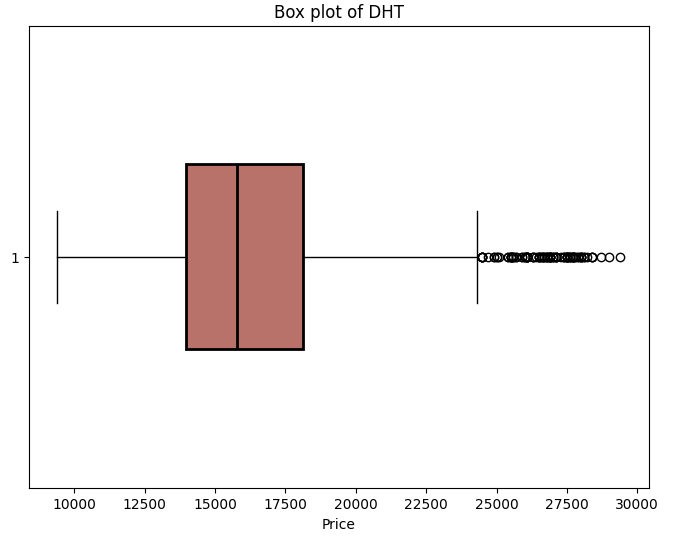
\includegraphics[width=1\textwidth]{bibliography/Figure/DHTboxplot.png}
    \caption{DHT stock price's boxplot}
    \label{fig:1}
    \end{minipage}
    \hfill
    \begin{minipage}{0.23\textwidth}
    \centering
    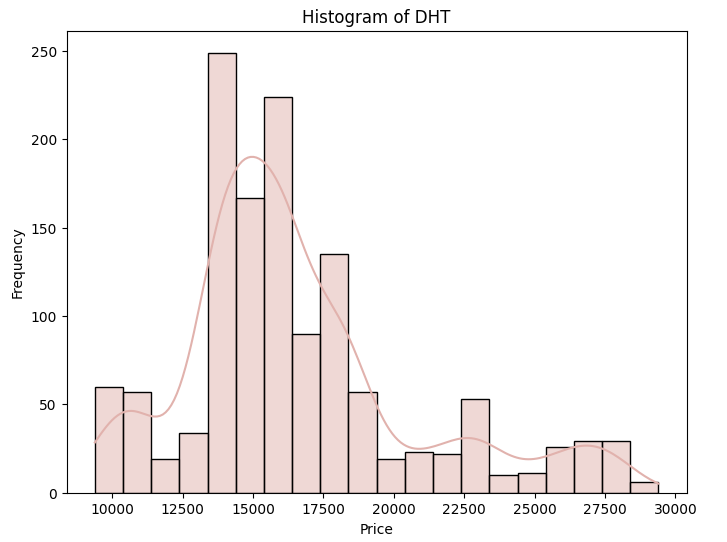
\includegraphics[width=1\textwidth]{bibliography/Figure/DHThist.png}
    \caption{DHT stock price's histogram}
    \label{fig:2}
    \end{minipage}
\end{figure}

\begin{figure}[H]
    \centering
    \begin{minipage}{0.23\textwidth}
    \centering
    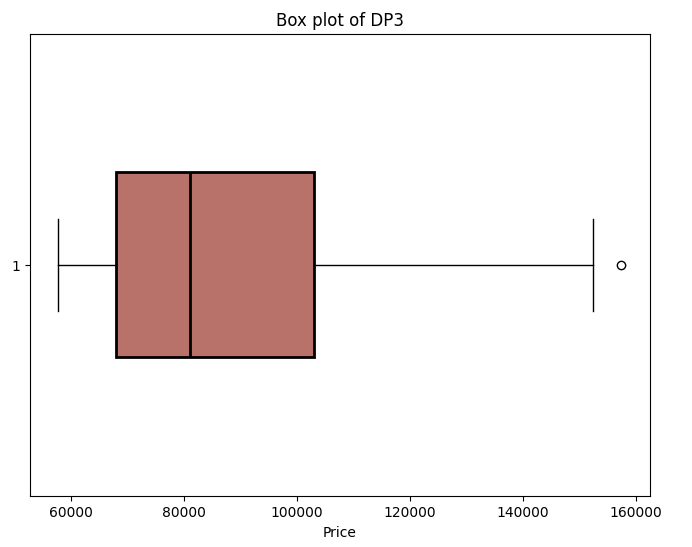
\includegraphics[width=1\textwidth]{bibliography/Figure/DP3boxplot.png}
    \caption{DP3 stock price's boxplot}
    \label{fig:1}
    \end{minipage}
    \hfill
    \begin{minipage}{0.23\textwidth}
    \centering
    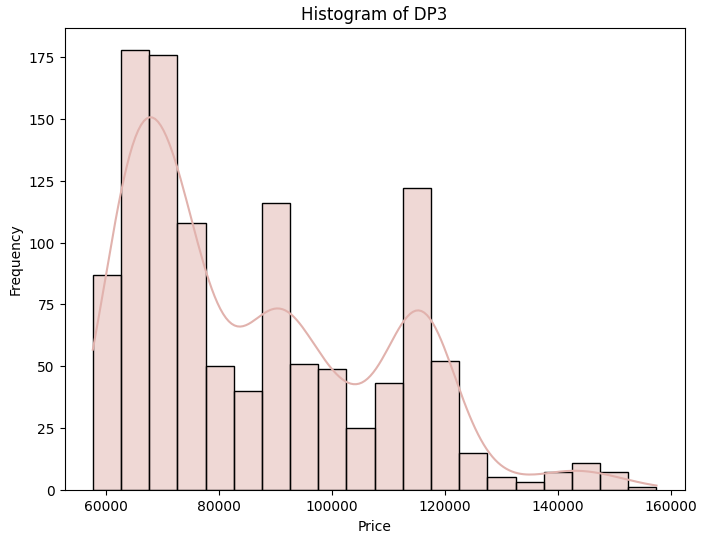
\includegraphics[width=1\textwidth]{bibliography/Figure/DP3hist.png}
    \caption{DP3 stock price's histogram}
    \label{fig:2}
    \end{minipage}
\end{figure}

\begin{figure}[H]
    \centering
    \begin{minipage}{0.23\textwidth}
    \centering
    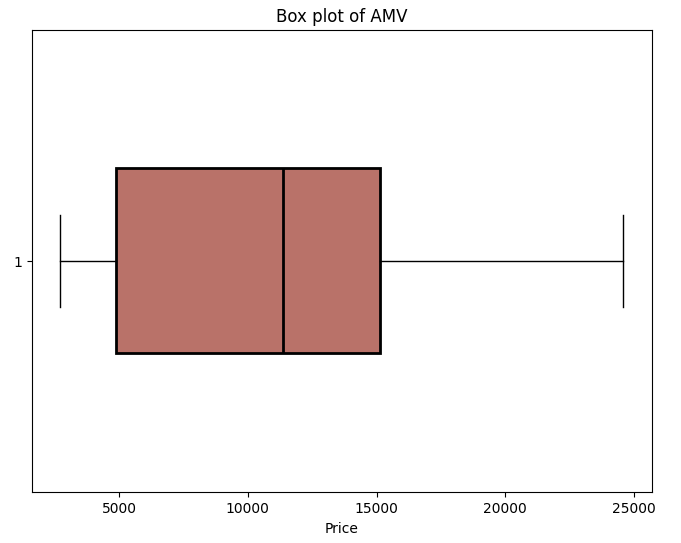
\includegraphics[width=1\textwidth]{bibliography/Figure/AMVboxplot.png}
    \caption{AMV stock price's boxplot}
    \label{fig:1}
    \end{minipage}
    \hfill
    \begin{minipage}{0.23\textwidth}
    \centering
    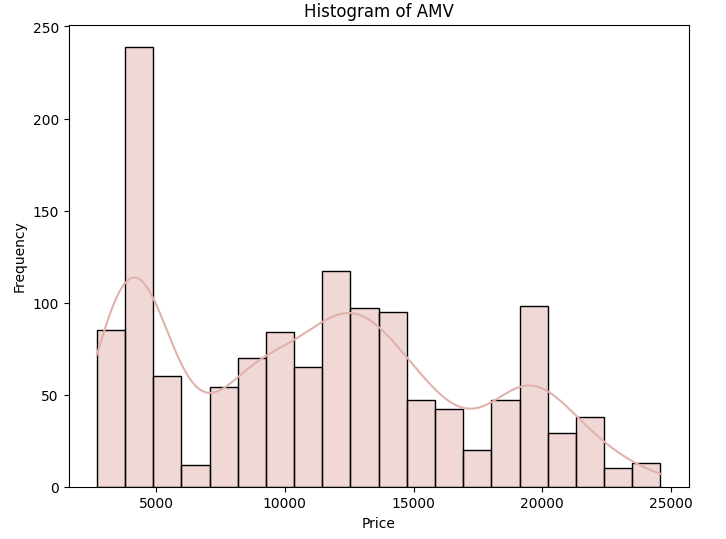
\includegraphics[width=1\textwidth]{bibliography/Figure/AMVhist.png}
    \caption{AMV stock price's histogram}
    \label{fig:2}
    \end{minipage}
\end{figure}
\section{Methodology}
\subsection{Linear Regression}
Regression analysis is a tool for building mathematical and statistical models that characterize relationships between a dependent variable and one or more independent, or explanatory, variables, all of which are numerical. This statistical technique is used to find an equation that best predicts the y variable as a linear function of the x variables.
A multiple linear regression model has the form: 
\[Y=\beta_0+\beta_1X_1+\beta_2X_2+\cdots+\beta_kX_k+\varepsilon\]
Where:\\
	\indent\textbullet\ Y is the dependent variable (Target Variable).\\
	\indent\textbullet\ \(X_1, X_2, \ldots, X_k\) are the independent (explanatory) variables.\\
	\indent\textbullet\ \(\beta_0\) is the intercept term.\\
	\indent\textbullet\ \(\beta_1,..., \beta_k\) are the regression coefficients for the independent variables.\\
	\indent\textbullet\ \(\varepsilon\) is the error term.

  \begin{figure}[H]
    \centering
    \begin{minipage}{0.8\linewidth}
      \centering
      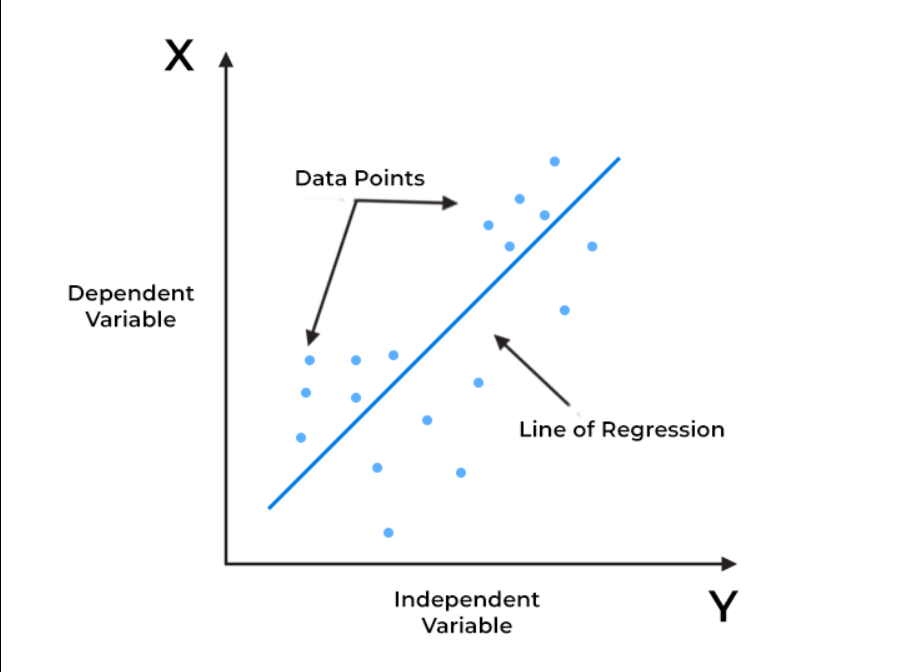
\includegraphics[width=\linewidth]{bibliography/Figure/LN_model.png}
      \caption{LN model's}
      \label{fig8}
    \end{minipage}
  \end{figure}

\subsection{Fast Fourier Transform }
The Fast Fourier Transform (FFT) is a method that allows computing the Discrete Fourier Transform (DFT) in $\mathcal{O}(n \log n)$ time. The basic idea of the FFT is to apply the divide-and-conquer approach. We divide the coefficient vector of the polynomial into two vectors, recursively compute the DFT for each of them, and combine the results to compute the DFT of the complete polynomial.

Let there be a polynomial $A(x)$ with degree $n - 1$, where $n$ is a power of $2$, and $n > 1$:

\begin{equation*}
|A(x)| = a_0x^0 + a_1x^1 + \cdots + a_{n-1}x^{n-1}
\end{equation*}

Where:

\begin{itemize}
    \item $|A(x)|$ is the absolute value of the polynomial $A(x)$.
    \item $a_0, a_1, \ldots, a_{n-1}$ are the coefficients of the polynomial.
    \item $x^0, x^1, \ldots, x^{n-1}$ are the corresponding powers of the variable $x$ for each coefficient.
    \item $n - 1$ is the highest degree of the polynomial.
    \item The $\cdots$ (read as "and so on") represents the remaining terms in the sequence.
\end{itemize}

We divide it into two smaller polynomials, one containing only the coefficients of the even positions, and the other containing the coefficients of the odd positions:

\begin{align*}
A_0(x) &= a_0x^0 + a_2x^1 + \cdots + a_{n-2}x^{\frac{n}{2}-1}\\
A_1(x) &= a_1x^0 + a_3x^1 + \cdots + a_{n-1}x^{\frac{n}{2}-1}
\end{align*}

In the FFT computation, we apply the divide-and-conquer approach recursively to the polynomials $A_0(x)$ and $A_1(x)$, and combine the results to obtain the DFT of the original polynomial $A(x)$. Dividing the polynomial into smaller polynomials and computing recursively significantly reduces the computational time compared to the traditional DFT computation method.

\subsection{ARIMA }
The ARIMA model (an acronym for Auto-Regressive Integrated Moving Average), essentially creates a linear equation which describes and forecasts your time series data. This equation is generated through three separate parts which can be described as:

•	AR — auto-regression: equation terms created based on past data points.

•	I — integration or differencing: accounting for overall “trend” in the data.

•	MA — moving average: equation terms of error or noise based on past data points.

An ARIMA model is characterized by 3 terms: p, d, q
where,

•	p is the order of the AR term.

•	q is the order of the MA term.

•	d is the number of differencing required to make the time series stationary.

A pure Auto Regressive (AR only) model is one where $Yt$ depends only on its own lags. That is, $Yt$ is a function of the ‘lags of $Yt$’.
\begin{equation*}
 Y_t = a + B_1 Y_{t-1} + B_2 Y_{t-2} + \ldots + B_p Y_{t-p} + \varepsilon_t
\end{equation*}

Where:

\begin{itemize}
    \item $Y_t$: The value of the time series at time $t$.
    \item $a$: A constant term.
    \item $B_1, B_2, \ldots, B_p$: Autoregressive coefficients representing the relationship between the current observation and its past values at lag intervals.
    \item $p$: The order of the autoregressive component.
    \item $\varepsilon_t$: A white noise error term at time $t$.
\end{itemize}
Likewise a pure Moving Average (MA only) model is one where Yt depends only on the lagged forecast errors.
\begin{equation*}
Y_t = a + \phi_1 \varepsilon_{t-1} + \phi_2 \varepsilon_{t-2} + \ldots + \phi_q \varepsilon_{t-q} + \varepsilon_t
\end{equation*}

Where:

\begin{itemize}
    \item $q$: The order of the moving average component.
\end{itemize}

An ARIMA model is one where the time series was differenced at least once to make it stationary and you combine the AR and the MA terms. So the equation becomes:

\begin{equation*}
Y_t = a + \sum_{i=1}^{p} \phi_i Y_{t-i} + \varepsilon_t + \sum_{j=1}^{q} B_j \varepsilon_{t-j}
\end{equation*}

To find the orders of AR, I, and MA components in an ARIMA model, analysts use ACF and PACF plots. A decreasing ACF suggests a MA component, with the lag where it drops below a threshold indicating its order. Significant spikes in PACF imply an AR component, with the lag where PACF cuts off after a spike revealing its order. By interpreting these plots, analysts select suitable orders for ARIMA modeling.

\subsection{LSTM}
Long Short-Term Memory (LSTM) network is a type of recurrent neural network (RNN) capable of learning long-term dependencies. The LSTM model consists of several components, including gates that control the flow of information through the network. The LSTM model can be described as follows:

\begin{itemize}
    \item Let $\mathbf{x}_t$ be the input vector at time step $t$.
    \item Let $\mathbf{h}_t$ be the hidden state vector at time step $t$.
    \item Let $\mathbf{c}_t$ be the cell state vector at time step $t$.
    \item Let $\mathbf{W}$, $\mathbf{U}$, and $\mathbf{b}$ be the weight matrices and bias vectors.
\end{itemize}

The LSTM model is defined by the following equations:

1. \textbf{Forget Gate:}
\[
\mathbf{f}_t = \sigma(\mathbf{W}_f \mathbf{x}_t + \mathbf{U}_f \mathbf{h}_{t-1} + \mathbf{b}_f)
\]

2. \textbf{Input Gate:}
\[
\mathbf{i}_t = \sigma(\mathbf{W}_i \mathbf{x}_t + \mathbf{U}_i \mathbf{h}_{t-1} + \mathbf{b}_i)
\]

3. \textbf{Candidate Memory Cell:}
\[
\mathbf{\tilde{c}}_t = \tanh(\mathbf{W}_c \mathbf{x}_t + \mathbf{U}_c \mathbf{h}_{t-1} + \mathbf{b}_c)
\]

4. \textbf{Cell State:}
\[
\mathbf{c}_t = \mathbf{f}_t \odot \mathbf{c}_{t-1} + \mathbf{i}_t \odot \mathbf{\tilde{c}}_t
\]

5. \textbf{Output Gate:}
\[
\mathbf{o}_t = \sigma(\mathbf{W}_o \mathbf{x}_t + \mathbf{U}_o \mathbf{h}_{t-1} + \mathbf{b}_o)
\]

6. \textbf{Hidden State:}
\[
\mathbf{h}_t = \mathbf{o}_t \odot \tanh(\mathbf{c}_t)
\]

Where:
\begin{itemize}
    \item $\sigma$ denotes the sigmoid activation function.
    \item $\tanh$ denotes the hyperbolic tangent activation function.
    \item $\odot$ denotes element-wise multiplication.
    \item $\mathbf{W}_f, \mathbf{W}_i, \mathbf{W}_c, \mathbf{W}_o$ are the input weight matrices.
    \item $\mathbf{U}_f, \mathbf{U}_i, \mathbf{U}_c, \mathbf{U}_o$ are the recurrent weight matrices.
    \item $\mathbf{b}_f, \mathbf{b}_i, \mathbf{b}_c, \mathbf{b}_o$ are the bias vectors.
    \item $\mathbf{f}_t$ is the forget gate vector.
    \item $\mathbf{i}_t$ is the input gate vector.
    \item $\mathbf{\tilde{c}}_t$ is the candidate memory cell vector.
    \item $\mathbf{c}_t$ is the cell state vector.
    \item $\mathbf{o}_t$ is the output gate vector.
    \item $\mathbf{h}_t$ is the hidden state vector.
\end{itemize}

\begin{figure}[H]
  \centering
  \begin{minipage}{0.8\linewidth}
    \centering
    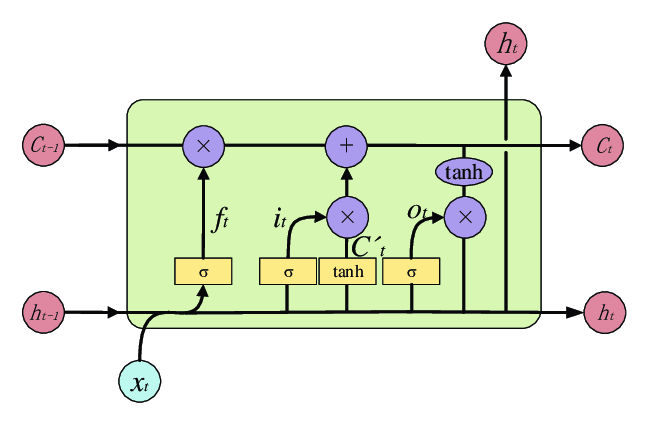
\includegraphics[width=\linewidth]{bibliography/Figure/LSTM_model.png}
    \caption{LSTM model's}
    \label{fig8}
  \end{minipage}
\end{figure}

\subsection{Linear Regression combined with CalendarFourier and DeterministicProcess }

Linear Regression combined with CalendarFourier and DeterministicProcess is an extended linear regression method used for modeling and forecasting time series with recurring cycles and growth trends. This method combines the following elements: 

\textbf{Linear Regression}:

\begin{itemize}
    \item Linear Regression is a common statistical modeling technique used to explore the linear relationship between an output variable (dependent variable) and one or more input variables (independent variables).
    \item Linear Regression is often used as a foundation for other time series forecasting techniques due to its ability to effectively model linear relationships.
\end{itemize}
\textbf{CalendarFourier}:

\begin{itemize}
    \item CalendarFourier is a time feature used to model recurring patterns in time series data.
    \item It transforms time into Fourier functions (sine and cosine), allowing the model to learn cyclical patterns such as daily, weekly, monthly, or yearly cycles.
    \item When combined with Linear Regression, CalendarFourier enhances the ability to forecast recurring cycles in time series data.
\end{itemize}
\textbf{DeterministicProcess}:

\begin{itemize}
    \item DeterministicProcess is a time feature used to model trends or growth patterns in time series data.
    \item It transforms time into a growth function (e.g., straight line, curve, polynomial, etc.), allowing the model to learn the long-term growth or decline trends of the data.
    \item When combined with Linear Regression, DeterministicProcess improves the ability to forecast long-term trends in time series data.
\end{itemize}
 
Suppose we have a time series \verb|y| and input variables \verb|X|. The Linear Regression model combined with CalendarFourier and DeterministicProcess takes the form: 

$$y = \beta_0 + \beta_1X_1 + \beta_2X_2 + ... + \beta_nX_n + f(t) + g(t) + \epsilon$$

Where:

\begin{itemize}
    \item \verb|y| is the output variable (the time series to be predicted).
    \item $\beta_0$ is the constant term.
\item $\beta_1, \beta_2, ..., \beta_n$ are the regression coefficients for the input variables $X_1, X_2, ..., X_n$.
    \item \verb|f(t)| is the CalendarFourier component, representing the recurring cycles in the time series, with \verb|t| being the time.
    \item \verb|g(t)| is the DeterministicProcess component, representing the growth trend in the time series, with \verb|t| being the time.
\item $\epsilon$ is the random error term.
\end{itemize}

 The CalendarFourier component \verb|f(t)| can be represented as a sum of sine and cosine functions with different cycle frequencies: 
 
$$f(t) = \alpha_1\sin(\omega t) + \beta_1\cos(\omega t) + \alpha_2\sin(2\omega t) + \beta_2\cos(2\omega t) + ... + $$

$$\alpha_k\sin(k\omega t) + \beta_k\cos(k\omega t)$$

 Where:

\begin{itemize}
\item $\omega$ is the cycle frequency (e.g., $2\pi/365$ for an annual cycle).
    \item $k$ is the number of Fourier terms used to model the cycles.
\item $\alpha_1, \beta_1, \alpha_2, \beta_2, ..., \alpha_k, \beta_k$ are the coefficients to be estimated from the data.
\end{itemize}


The DeterministicProcess component \verb|g(t)| can be represented by a growth function, such as a polynomial, exponential, or logarithmic function:

 $$g(t) = \gamma_1t + \gamma_2t^2 + \gamma_3t^3 + ... \quad \text{(polynomial)}$$
$$g(t) = \gamma_1 + \gamma_2\log(t) \quad \text{(logarithmic)}$$
$$g(t) = \gamma_1\exp(\gamma_2t) \quad \text{(exponential)}$$

Where $\gamma_1, \gamma_2, \gamma_3, ...$ are the coefficients to be estimated from the data.

The estimation of the coefficients $\beta_0, \beta_1, \beta_2, ..., \beta_n, \alpha_1, \beta_1, \alpha_2, \beta_2, ..., \alpha_k, \beta_k, \gamma_1, \gamma_2, \gamma_3, ...$ can be performed using the Ordinary Least Squares (OLS) method or other optimization techniques.

 By combining these components, the Linear Regression model with CalendarFourier and DeterministicProcess can effectively model and forecast both recurring cycles and growth trends in the time series, thereby achieving higher forecasting accuracy compared to simpler models. 
 
 \subsection{Gated Recurrent Unit}
 The Gated Recurrent Unit (GRU) is a type of recurrent neural network (RNN) architecture similar to Long Short-Term Memory (LSTM) but with a simpler design and fewer parameters. GRU employs two gates: the reset gate and the update gate. The reset gate controls the forgetting of the previous hidden state, while the update gate manages the incorporation of a candidate activation vector into the new hidden state.

 The GRU processes sequential data one element at a time, updating its hidden state based on the current input and the previous hidden state. At each time step, it computes a "candidate activation vector" that combines information from the input and previous hidden state. This vector is updated using the reset gate, which controls how much of the previous hidden state to forget, and the update gate, which determines how much of the candidate activation vector to incorporate into the new hidden state.

 Here’s the math behind the GRU architecture:

 1. The reset gate \( r \) and update gate \( z \) are computed using the current input \( x \) and the previous hidden state \( h_{t-1} \):

 \[
  r_t = \text{sigmoid}(\mathbf{W}_r \cdot [h_{t-1}, x_t])
  \]
  \[
  z_t = \text{sigmoid}(\mathbf{W}_z \cdot [h_{t-1}, x_t])
  \]

where \( \mathbf{W}_r \) and \( \mathbf{W}_z \) are weight matrices that are learned during training.

 2. The candidate activation vector \( \tilde{h}_t \) is computed using the current input \( x \) and a modified version of the previous hidden state that is "reset" by the reset gate:

\[ \tilde{h}_t = \frac{{e^{r_t \ast h_{t-1}} + e^{-r_t \ast h_{t-1}}}}{{e^{r_t \ast h_{t-1}} - e^{-r_t \ast h_{t-1}}}} \cdot x_t \]

where \( \mathbf{W}_h \) is another weight matrix.

 3. The new hidden state \( h_t \) is computed by combining the candidate activation vector with the previous hidden state, weighted by the update gate:

\[ h_t = (1 - z_t) \ast h_{t-1} + z_t \ast \tilde{h}_t \]

 Overall, the reset gate controls the retention of the previous hidden state, and the update gate determines how much of the candidate activation vector updates the new hidden state. This compact architecture selectively updates its hidden state without needing a separate memory cell like LSTM.
 \subsection{LightGBM}
 LightGBM, short for Light Gradient Boosting Machine, is a gradient boosting framework developed by Microsoft. It’s renowned for its efficiency and speed. The fundamental representation of how LightGBM combines predictions from different trees to make a final prediction can be represented by the following formula:

\[ 
Y = \text{Base\_tree}(X) - \text{lr} \times \text{Tree}_{1}(X) - \text{lr} \times \text{Tree}_{2}(X) - \text{lr} \times \text{Tree}_{3}(X) 
\]

 Here, Y is the final prediction, Base tree(X) is the prediction of the base model, Tree1(X), Tree2(X), and Tree3(X) are the predictions of subsequent models, and lr is the learning rate

 LightGBM introduces two key techniques: Gradient-based One-Side Sampling (GOSS) and Exclusive Feature Bundling (EFB).
 
 \begin{itemize}
    \item GOSS focuses on sampling instances based on their gradients, prioritizing those with larger gradients for training. It also randomly drops instances with small gradients, thereby reducing the computational burden.
    \item EFB optimizes memory usage by bundling exclusive features together, allowing for more efficient processing and faster training without compromising the performance significantly.
 \end{itemize}

 LightGBM employs histogram-based algorithms to find the best split points during tree construction1. Instead of exhaustively searching through all possible split points, LightGBM discretizes continuous features into discrete bins and constructs histograms to approximate the optimal split points. This approach significantly reduces computational complexity and memory usage, especially for datasets with a large number of unique feature values.

 \begin{figure}[H]
  \centering
  \begin{minipage}{0.8\linewidth}
    \centering
    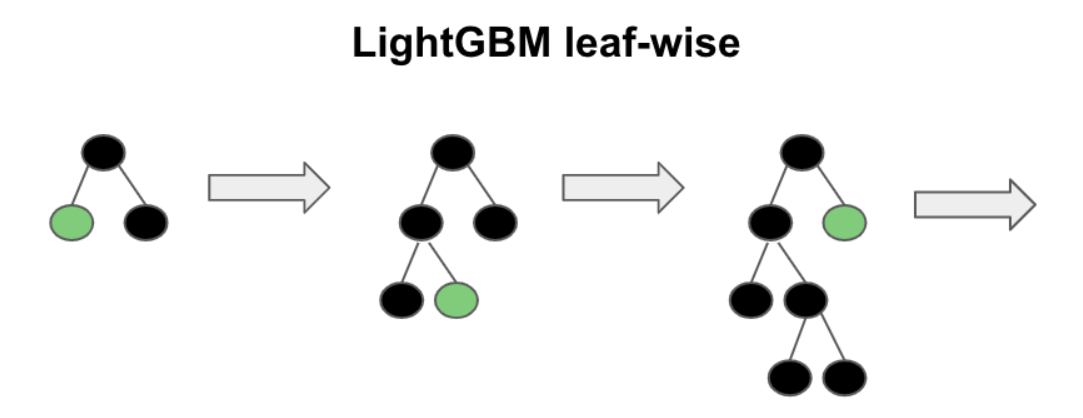
\includegraphics[width=\linewidth]{bibliography/Figure/LightGBM_model.png}
    \caption{LightGBM model's}
    \label{fig8}
  \end{minipage}
\end{figure}
 
\subsection{Recurrent Neural Network}
Recurrent Neural Network (RNN) is a neural network architecture that enables processing sequential data in O(n) time complexity. The core idea of RNNs is to apply the divide-and-conquer approach. We divide the input sequence into time steps, recursively compute for each step, and combine the results to process the complete input sequence. 
Let $X$ be an input sequence of length $n$:
\begin{equation}
  |X| = x_1, x_2, ..., x_n
  \end{equation}
  Where:
  \begin{itemize}
  \item $|X|$ is the length of the input sequence $X$.
  \item $x_1, x_2, ..., x_n$ are the elements of the sequence.
  \item ... (read as "and so on") represents the remaining elements in the sequence.
  \end{itemize}
  We divide the input sequence into time steps, processing one element at each step:
  \begin{align}
  h_1 &= f(x_1, h_0) \
  h_2 &= f(x_2, h_1) \
  &...\
  h_n &= f(x_n, h_{n-1})
  \end{align}
  In which:
  \begin{itemize}
  \item $h_t$ is the hidden state at time step $t$.
  \item $f$ is a computation function, typically a non-linear transformation (e.g., tanh, ReLU) of the linear combination of the input $x_t$ and the previous hidden state $h_{t-1}$.
  \item $h_0$ is the initial hidden state, usually initialized as zeros.
  \end{itemize}

  In the RNN computation, we apply the divide-and-conquer approach recursively at each time step, computing the hidden state $h_t$ based on the input $x_t$ and the previous hidden state $h_{t-1}$. The final result is the hidden state $h_n$, which encapsulates the contextual information from the entire input sequence.

  The output $y_t$ at each time step $t$ is computed based on the current hidden state $h_t$ and input $x_t$, typically through an output layer:
  \begin{equation}
  y_t = g(h_t, x_t)
  \end{equation}
  Where $g$ is a function, often a linear transformation or a neural network.

  Recurrent structure allows RNNs to capture long-range dependencies within the sequential data, making them suitable for various tasks such as language modeling, machine translation, speech recognition, and time series prediction.
\section{Result}
\subsection{Evaluation Methods}
\textbf{Mean Percentage Absolute Error} (MAPE): is the average percentage error in a set of predicted values.\\
\[MAPE=\frac{100\%}{n}  \sum_{i=1}^{n} |y_i-\hat{y_i} |  = 1 \]\\
\textbf{Root Mean Squared Error} (RMSE): is the square root of average value of squared error in a set of predicted values.\\
\[RMSE=\sqrt{\sum_{i=1}^{n} \frac{(\hat{y_i}-y_i )^2}{n} }\]\\
\textbf{Mean Absolute Error} (MSLE):is the relative difference between the log-transformed actual and predicted values.\\
\[MSLE=\frac{1}{n}\sum_{i=1}^{n}(log(1+\hat{y_i})-log(log(1+y_i))^2\]
Where: \\
	\indent\textbullet\ \(n\) is the number of observations in the dataset.\\
	\indent\textbullet\ \(y_i\)  is the true value.\\
	\indent\textbullet\ \(\hat{y_i}\) is the predicted value.
\subsection{AMV Dataset} 
\begin{table}[H]
    \centering
    \begin{tabular}{|c|c|c|c|c|}
         \hline
         \multicolumn{5}{|c|}{\textbf{AMV Dataset's Evaluation}}\\
         \hline
         \centering Model & Training:Testing & RMSE & MAPE (\%) & MSLE\\
         \hline
         \multirow{2}{*}{LN}& 7:3 & 7787.57 & 0.4966\% & 0.1963\\ & 8:2 & 9121.15 & 0.6732\% & 0.2726\\ & \textbf{9:1}& 6901.35& 0.5173\% & 0.1753\\
         \hline
         \multirow{2}{*}{RNN} & 7:3&1276.19&0.3207&0.0801\\ & \textbf{8:2}&135.78&0.0264&0.0011\\ & 9:1  &264.547 &0.0665 &0.0054 \\
         \hline
         \multirow{2}{*}{GRU} & \textbf{7:3}	& & & \\ & 8:2 & & & \\ & 9:1 & & & \\
         \hline
         \multirow{2}{*}{ARIMA} & 7:3 & 558.44 & 11.50\% & 0.02 \\ & 8:2 & 801.64 & 18.26\% & 0.04 \\ & \textbf{9:1} & 290.25 & 5.51\% & 0.00\\
         \hline
         \multirow{2}{*}{FFT}& 7:3	& 0.0829& 4151& 0.0054\\ & 8:2 & 0.05950& 0.9657& 0.003\\ & \textbf{9:1} & 0.0259& 0.5279& 0.0006\\
         \hline
         \multirow{2}{*}{LN-CF-DP} & 7:3 & 6841.46 & 165.18\% & 0.96 \\ & 8:2 &2031.85	& 44.21\%&  0.15 \\ & \textbf{9:1} &1441.58&33.21\% & 0.10\\
         \hline
         \multirow{2}{*}{LSTM}& 7:3& 666.91& 0.0232\%& 0.0019\\ & 8:2 & 371.68& 0.0181\%& 0.0007\\ & \textbf{9:1}& 260.59& 0.0141\%& 0.0003\\
         \hline
         \multirow{2}{*}{LightGBM}& 7:3& 1149.51& 0.0593\% & 0.0057\\ & 8:2 & 681.00& 0.0380\% & 0.0022\\ & \textbf{9:1}& 417.32& 0.0263\% & 0.0009\\
         \hline
    \end{tabular}
    \caption{AMV Dataset's Evaluation}
    \label{vcbresult}
\end{table}

\begin{figure}[H]
  \centering
  \begin{minipage}{0.8\linewidth}
    \centering
    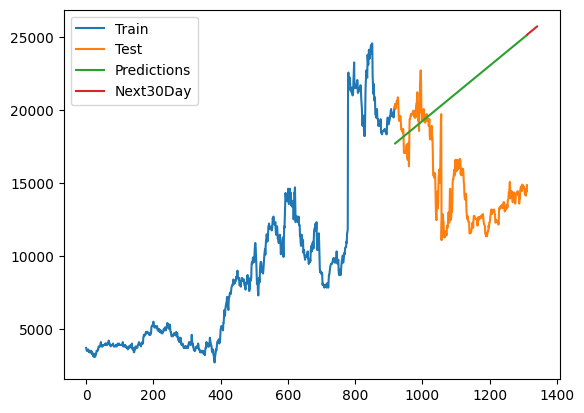
\includegraphics[width=\linewidth]{bibliography/Figure/LN_AMV(7_3).png}
    \caption{Linear model's result with 7:3 splitting proportion}
    \label{fig8}
  \end{minipage}
\end{figure}

\begin{figure}[H]
  \centering
  \begin{minipage}{0.8\linewidth}
    \centering
    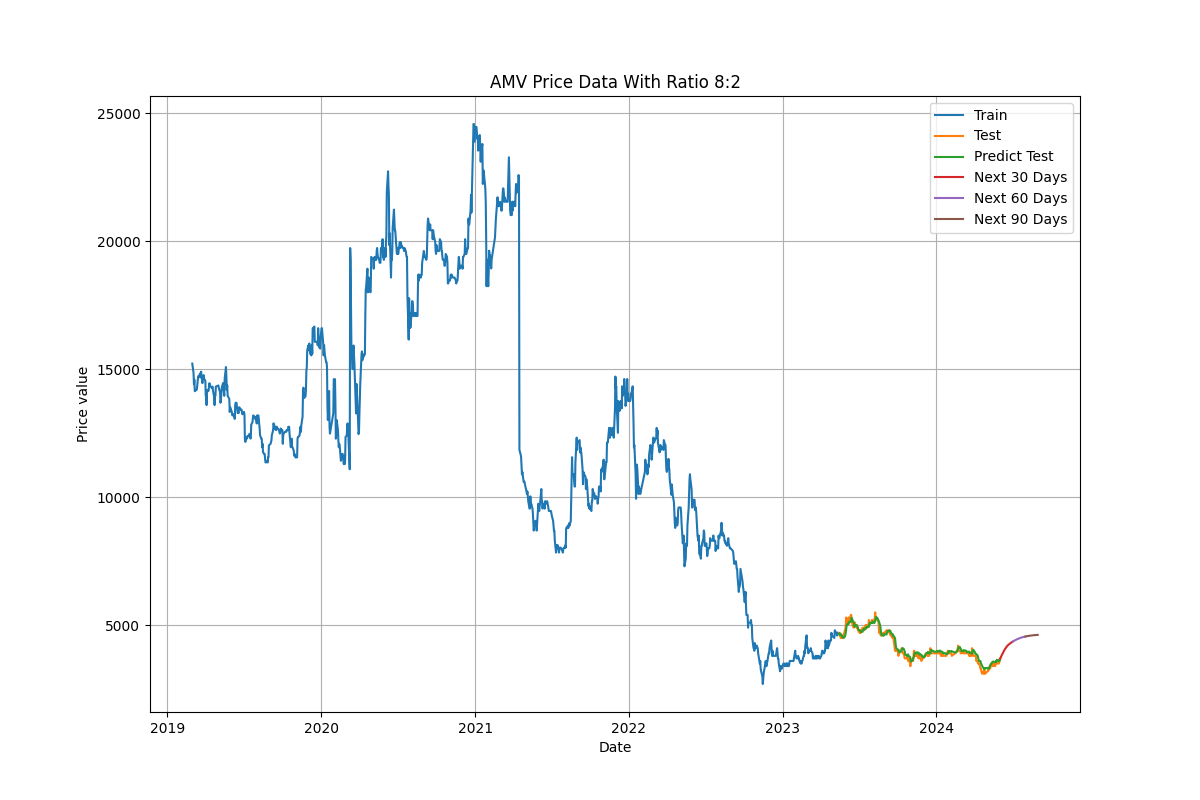
\includegraphics[width=\linewidth]{bibliography/Figure/RNN_82_AMV.png}
    \caption{RNN model's result with 8:2 splitting proportion}
    \label{fig8}
  \end{minipage}
\end{figure}


\begin{figure}[H]
  \centering
  \begin{minipage}{0.8\linewidth}
    \centering
    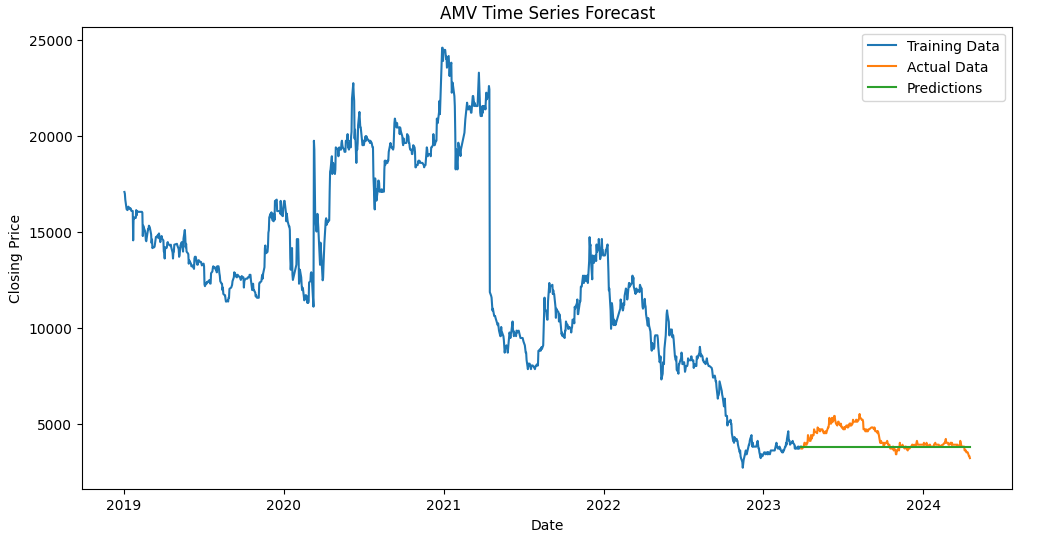
\includegraphics[width=\linewidth]{bibliography/Figure/AMV_ARIMA.png}
    \caption{Arima model's result with 8:2 splitting proportion}
    \label{fig8}
  \end{minipage}
\end{figure}

\begin{figure}[H]
  \centering
  \begin{minipage}{0.8\linewidth}
    \centering
    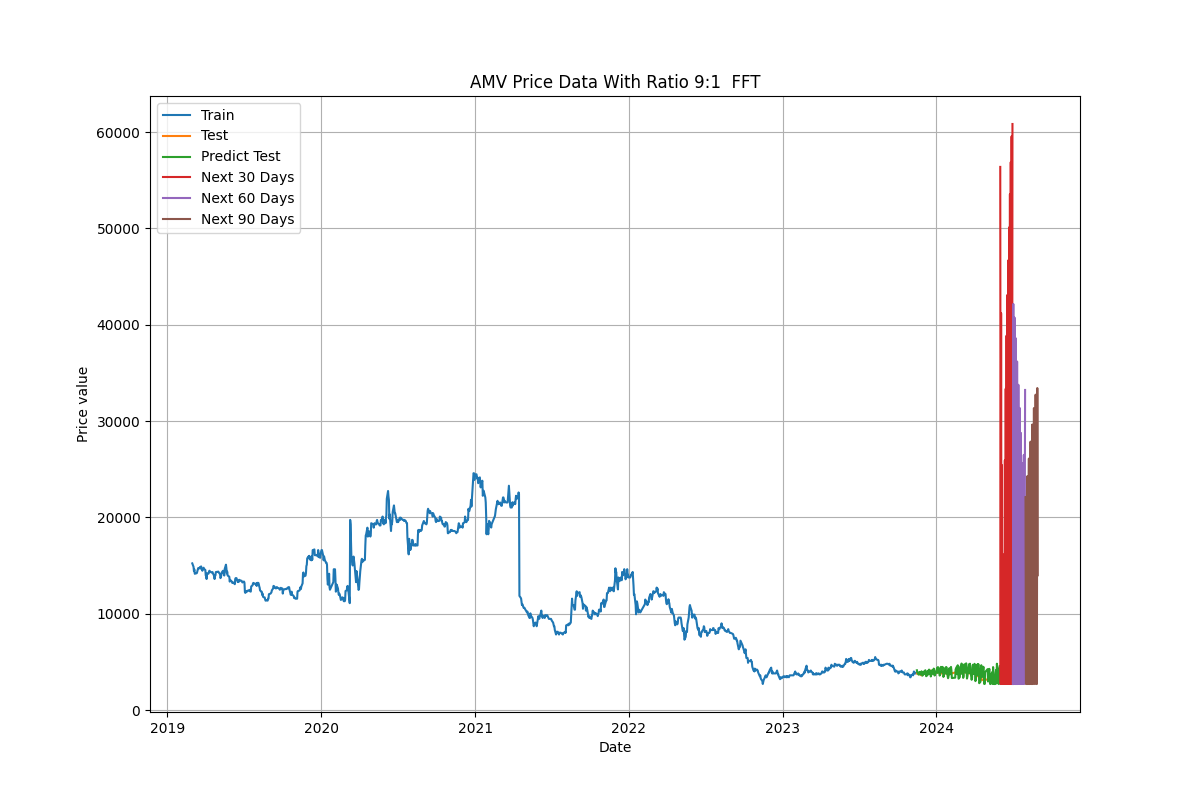
\includegraphics[width=\linewidth]{bibliography/Figure/FFT_91_AMV.png}
    \caption{FFT model's result with 9:1 splitting proportion}
    \label{fig8}
  \end{minipage}
\end{figure}

\begin{figure}[H]
  \centering
  \begin{minipage}{0.8\linewidth}
    \centering
    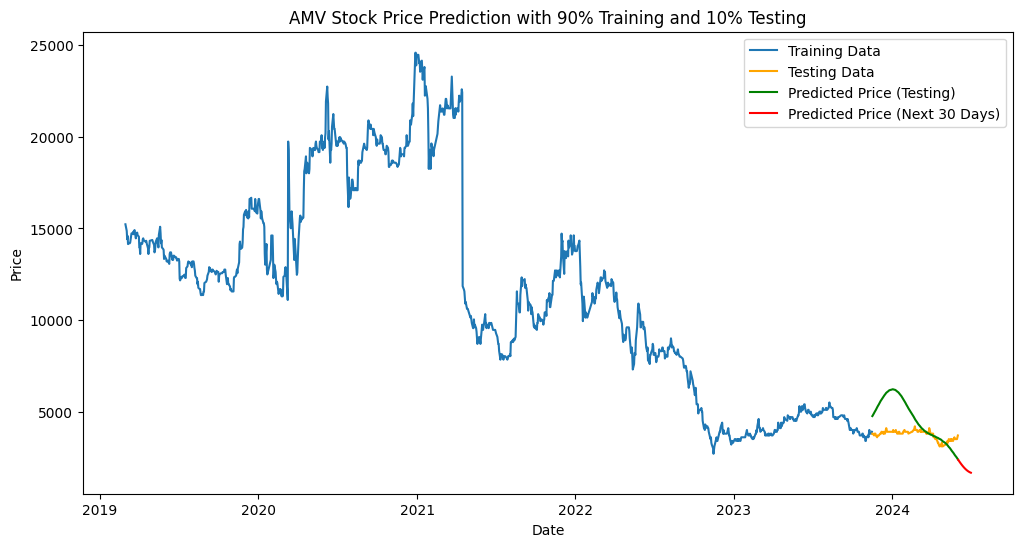
\includegraphics[width=\linewidth]{bibliography/Figure/AMV_LN_CF&DP.png}
    \caption{LN-CF-DP model's result with 9:1 splitting proportion}
    \label{fig8}
  \end{minipage}
\end{figure}

\begin{figure}[H]
  \centering
  \begin{minipage}{0.8\linewidth}
    \centering
    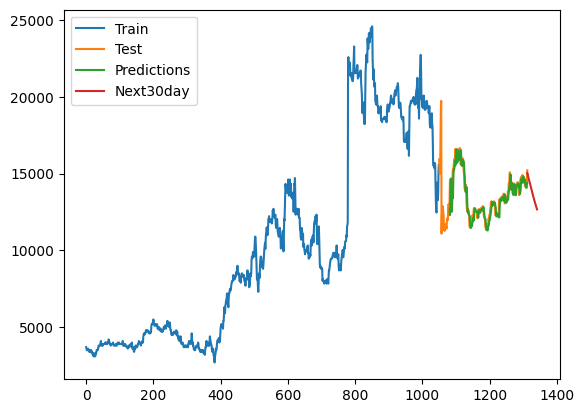
\includegraphics[width=\linewidth]{bibliography/Figure/LSTM_AMV(8_2).png}
    \caption{LSTM model's result with 8:2 splitting proportion}
    \label{fig8}
  \end{minipage}
\end{figure}

\begin{figure}[H]
  \centering
  \begin{minipage}{0.8\linewidth}
    \centering
    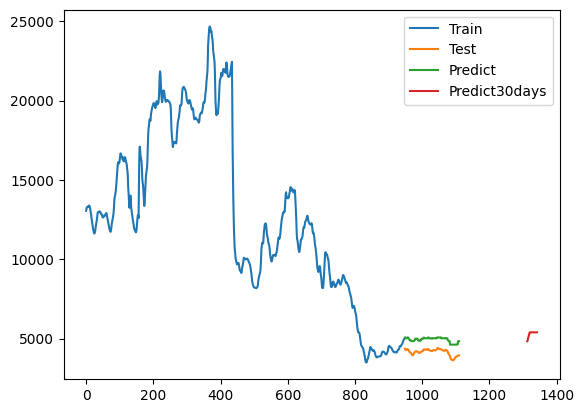
\includegraphics[width=\linewidth]{bibliography/Figure/LightGBM_AMV(8_2).png}
    \caption{LightGBM model's result with 8:2 splitting proportion}
    \label{fig8}
  \end{minipage}
\end{figure}

\begin{figure}[H]
  \centering
  \begin{minipage}{0.8\linewidth}
    \centering
    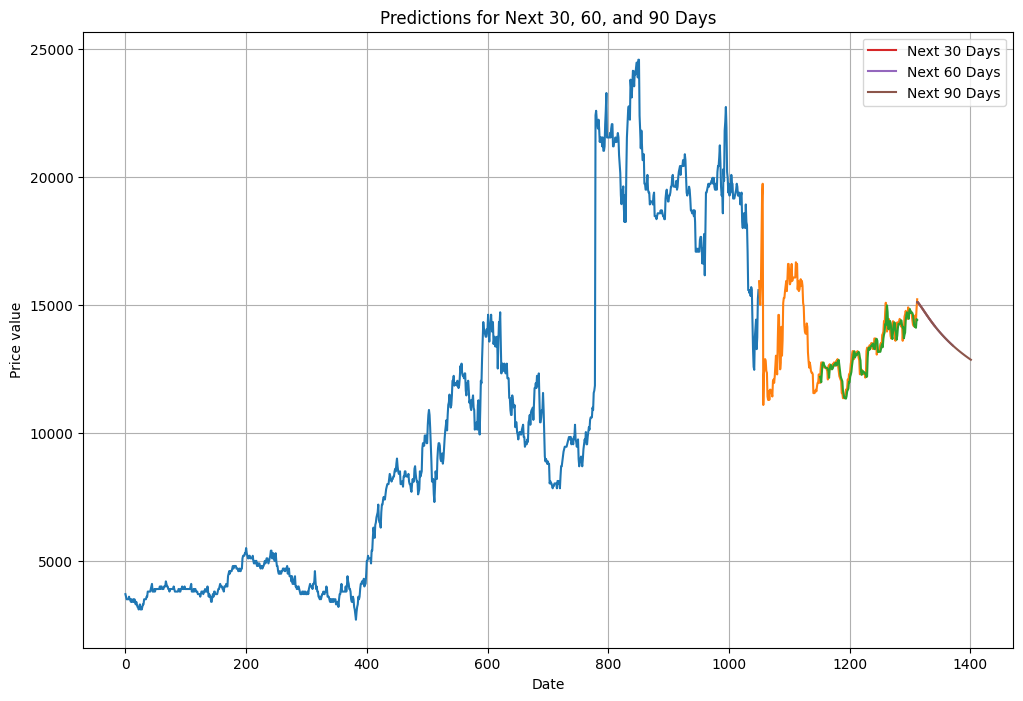
\includegraphics[width=\linewidth]{bibliography/Figure/AMV_GRU.png}
    \caption{GRU model's result with 8:2 splitting proportion}
    \label{fig8}
  \end{minipage}
\end{figure}

\subsection{DP3 Dataset}
\begin{table}[H]
    \centering
    \begin{tabular}{|c|c|c|c|c|}
         \hline
         \multicolumn{5}{|c|}{\textbf{DP3 Dataset's Evaluation}}\\
         \hline
         \centering Model & Training:Testing & RMSE & MAPE (\%) & MSLE\\
         \hline
         \multirow{2}{*}{LN}& 7:3 & 7787.57 & 0.4966\% & 0.1963\\ & 8:2 & 9121.15 & 0.6732\% & 0.2726\\ & \textbf{9:1}& 6901.35& 0.5173\% & 0.1753\\
         \hline
         \multirow{2}{*}{RNN} & 7:3&1675.09&0.0412&0.0037\\ & 8:2&2503.94&0.0700&0.0081\\ & \textbf{9:1} & 1499.11&0.0275 &0.0021 \\
         \hline
         \multirow{2}{*}{GRU} & \textbf{7:3}	& & & \\ & 8:2 & & & \\ & 9:1 & & & \\
         \hline
         \multirow{2}{*}{ARIMA} & 7:3 & 27750.14  & 39.01\%  &  0.36 \\ & 8:2 & 7936.36  & 10.027\% & 0.01 \\ & \textbf{9:1} & 6394.82 & 7.79\% & 0.01 \\
         \hline
         \multirow{2}{*}{FFT}& 7:3& 0.2076& 61.27\%&0.0232 \\ & 8:2 & 0.1987& 59.18\%& 0.0224\\ & \textbf{9:1}& 0.1352& 37.86\%& 0.0103\\
         \hline
         \multirow{2}{*}{LN-CF-DP} & 7:3 & 54681.37 & 69.13 & 0.31 \\ & {8:2} & 48774.18 & 67.56 & 0.28 \\ & \textbf{9:1} & 45471.00 &66.45&0.26\\
         \hline
         \multirow{2}{*}{LSTM}& 7:3& 2667.39& 0.0323\%& 0.0014\\ & 8:2 & 1495.67& 0.0152\%& 0.0004\\ & \textbf{9:1}& 1321.26& 0.0127\%& 0.0003\\
         \hline
         \multirow{2}{*}{LightGBM}& 7:3& 2281.21& 0.0254\% & 0.0010\\ & 8:2 & 1912.37& 0.0236\% & 0.0008\\ & \textbf{9:1}& 1765.80& 0.0203\% & 0.0006\\
         \hline
    \end{tabular}
    \caption{DP3 Dataset's Evaluation}
    \label{dp3result}
\end{table}

\begin{figure}[H]
  \centering
  \begin{minipage}{0.8\linewidth}
    \centering
    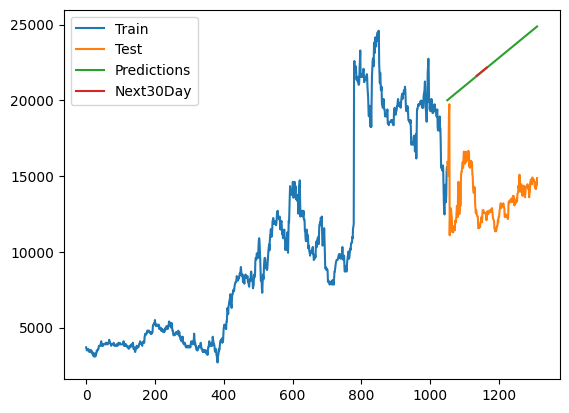
\includegraphics[width=\linewidth]{bibliography/Figure/LN_DP3(8_2).png}
    \caption{Linear model's result with 8:2 splitting proportion}
    \label{fig8}
  \end{minipage}
\end{figure}

\begin{figure}[H]
  \centering
  \begin{minipage}{0.8\linewidth}
    \centering
    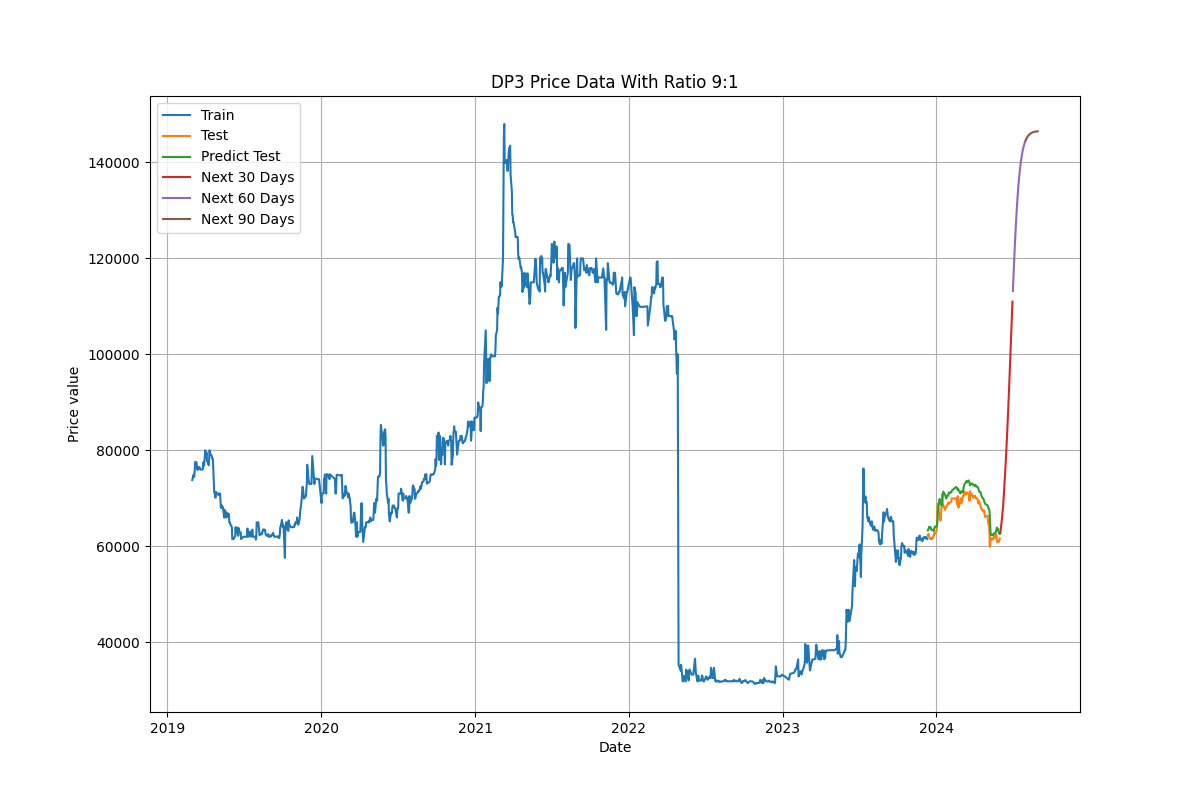
\includegraphics[width=\linewidth]{bibliography/Figure/RNN_91_DP3.png}
    \caption{RNN model's result with 9:1 splitting proportion}
    \label{fig8}
  \end{minipage}
\end{figure}

\begin{figure}[H]
  \centering
  \begin{minipage}{0.8\linewidth}
    \centering
    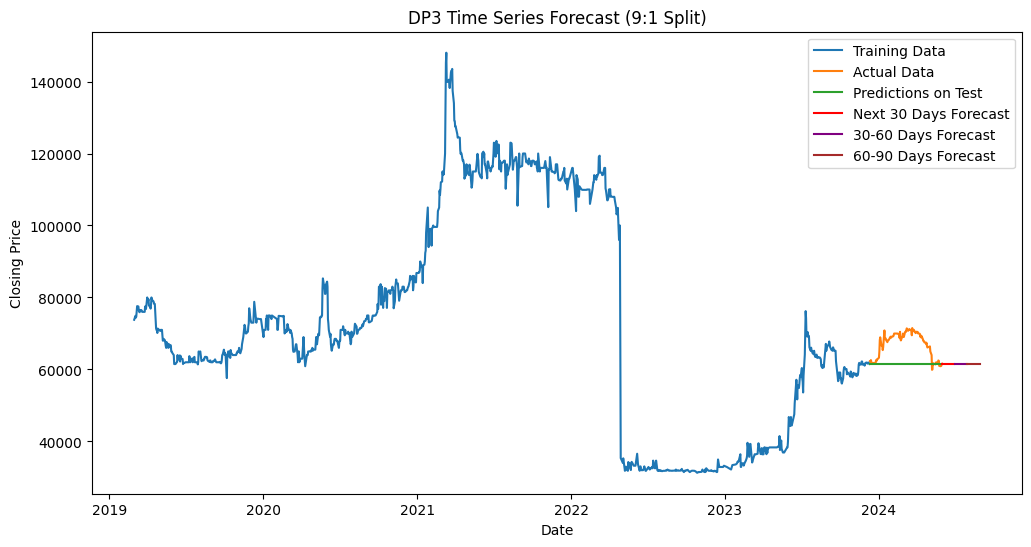
\includegraphics[width=\linewidth]{bibliography/Figure/DP3_ARIMA.png}
    \caption{ARIMA model's result with 8:2 splitting proportion}
    \label{fig8}
  \end{minipage}
\end{figure}

\begin{figure}[H]
  \centering
  \begin{minipage}{0.8\linewidth}
    \centering
    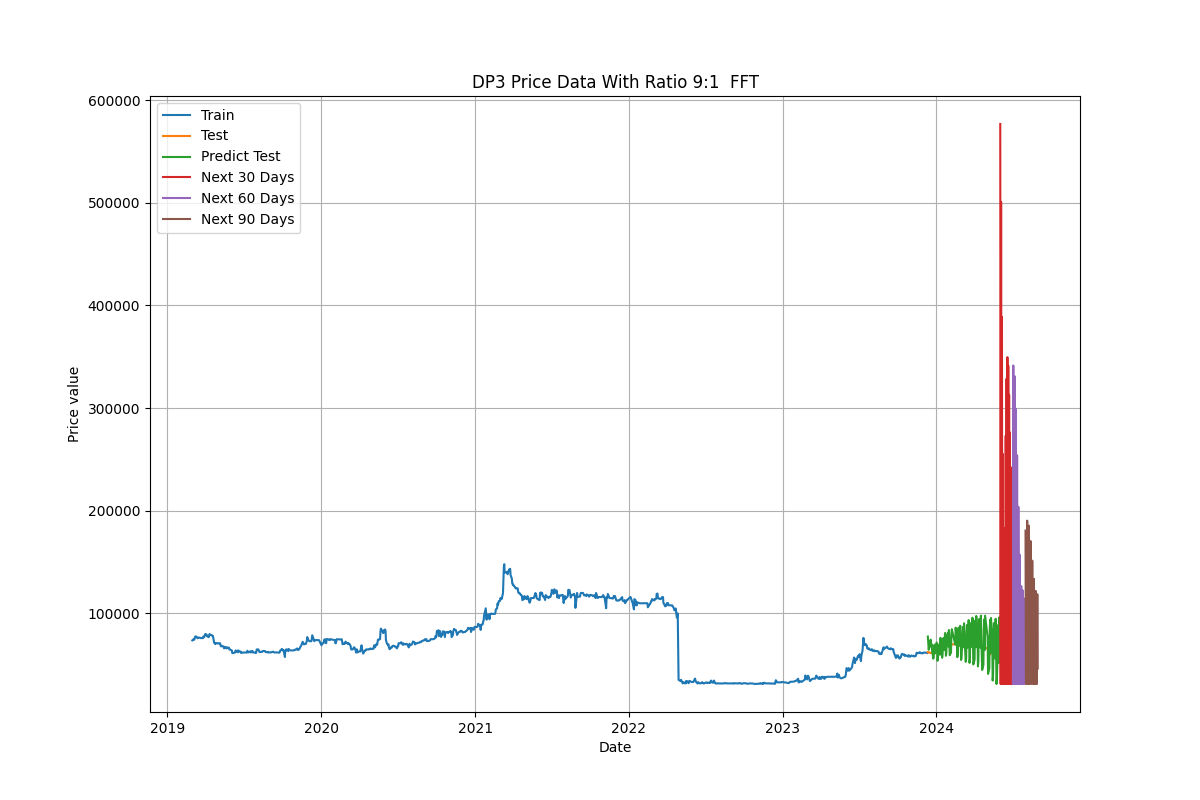
\includegraphics[width=\linewidth]{bibliography/Figure/FFT_91_DP3.png}
    \caption{FFT model's result with 9:1 splitting proportion}
    \label{fig8}
  \end{minipage}
\end{figure}

\begin{figure}[H]
  \centering
  \begin{minipage}{0.8\linewidth}
    \centering
    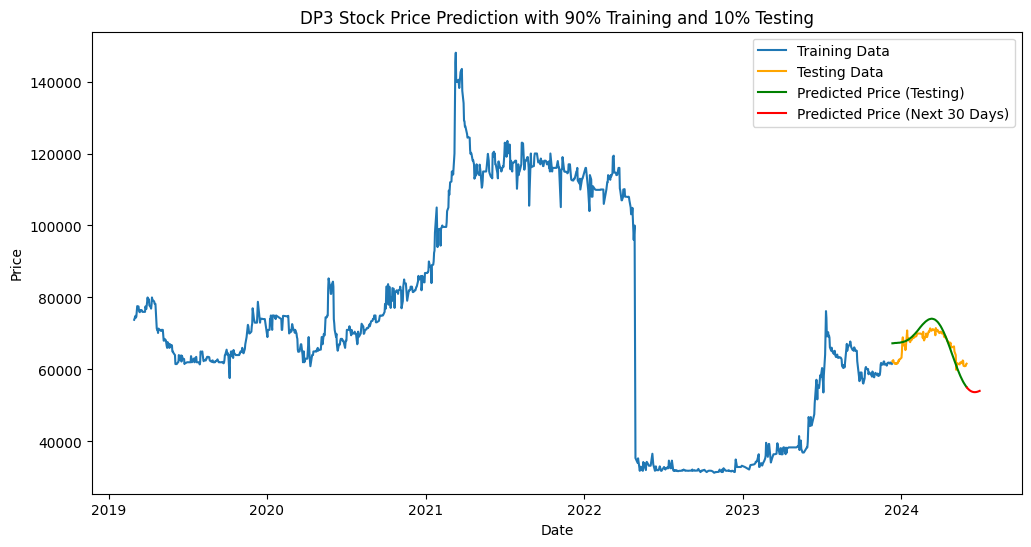
\includegraphics[width=\linewidth]{bibliography/Figure/DP3_LN_CF&DP.png}
    \caption{LN-CF-DP model's result with 9:1 splitting proportion}
    \label{fig8}
  \end{minipage}
\end{figure}

\begin{figure}[H]
  \centering
  \begin{minipage}{0.8\linewidth}
    \centering
    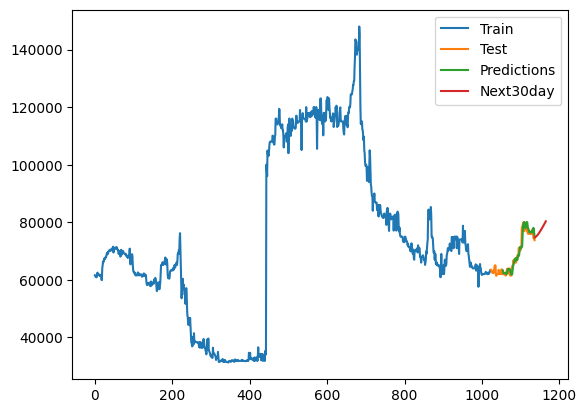
\includegraphics[width=\linewidth]{bibliography/Figure/LSTM_DP3(9_1).png}
    \caption{LSTM model's result with 9:1 splitting proportion}
    \label{fig8}
  \end{minipage}
\end{figure}

\begin{figure}[H]
  \centering
  \begin{minipage}{0.8\linewidth}
    \centering
    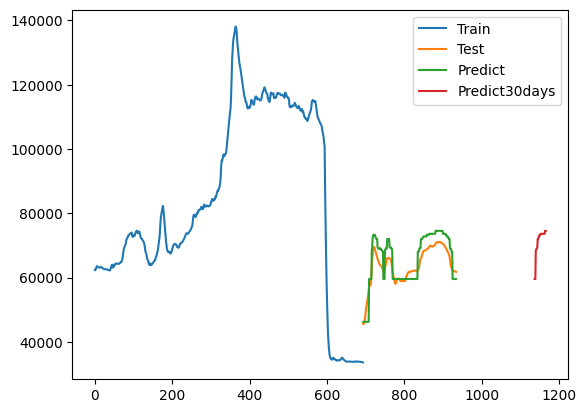
\includegraphics[width=\linewidth]{bibliography/Figure/LightGBM_DP3(7_3).png}
    \caption{LightGBM model's result with 7:3 splitting proportion}
    \label{fig8}
  \end{minipage}
\end{figure}

\begin{figure}[H]
  \centering
  \begin{minipage}{0.8\linewidth}
    \centering
    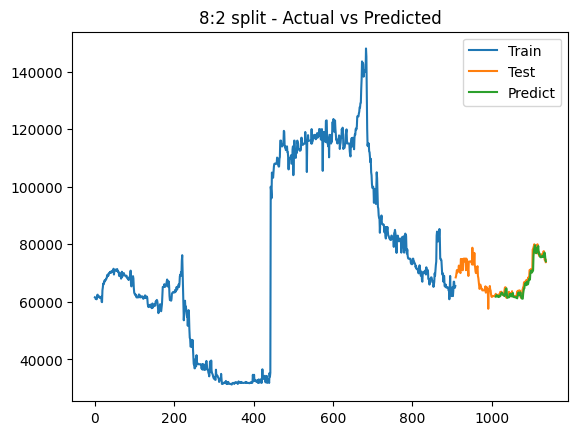
\includegraphics[width=\linewidth]{bibliography/Figure/DP3_GRU.png}
    \caption{GRU model's result with 9:1 splitting proportion}
    \label{fig8}
  \end{minipage}
\end{figure}

\subsection{DHT Dataset} 
\begin{table}[H]
    \centering
    \begin{tabular}{|c|c|c|c|c|}
         \hline
         \multicolumn{5}{|c|}{\textbf{DHT Dataset's Evaluation}}\\
         \hline
         \centering Model & Training:Testing & RMSE & MAPE (\%) & MSLE\\
         \hline
         \multirow{2}{*}{LN}& 7:3 & 7781.26 & 49.62 & 0.19\\ & 8:2 & 9119.01 & 67.34 & 0.27\\ & \textbf{9:1}& 6907.31& 51.82 & 0.17\\
         \hline
         \multirow{2}{*}{RNN} & 7:3&7787.57&0.4966\%&0.1963\\ & 8:2&9121.15&0.6732\%& 0.2726\\ & \textbf{9:1} &6901.35 &0.5173\% & 0.1753\\
         \hline
         \multirow{2}{*}{GRU} & \textbf{7:3}	& & & \\ & 8:2 & & & \\ & 9:1 & & & \\
         \hline
         \multirow{2}{*}{ARIMA} & 7:3 & 9640.50 & 29.78\% &0.24 \\ & 8:2 & 9305.45 &31.50\% & 0.18\\ & \textbf{9:1} &5570.55 &12.58\% & 0.04\\
         \hline
         \multirow{2}{*}{FFT}& 7:3	& 0.5714& 63.88\%& 0.0871\\ & 8:2 & 0.5188& 57.93\%& 0.0862\\ & \textbf{9:1} & 0.3351& 34.96\%& 0.3354\\
         \hline
         \multirow{2}{*}{LN-CF-DP} & \textbf{7:3} & 5726.49&24.00&0.08 \\ & {8:2} &8043.72& 29.24& 0.16\\ & 9:1 &6725.16&24.92&0.10\\
         \hline
         \multirow{2}{*}{LSTM}& 7:3& 684.28& 0.0368\%& 0.0022\\ & 8:2 & 550.75& 0.0295\%& 0.0017\\ & \textbf{9:1}& 519.76& 0.0412\%& 0.0023\\
         \hline
         \multirow{2}{*}{LightGBM}& 7:3& 2095.46& 0.1271\% & 0.0293\\ & 8:2 & 2543.66& 0.1783\% & 0.0440\\ & \textbf{9:1}& 3738.55& 0.3583\% & 0.0968\\
         \hline
    \end{tabular}
    \caption{DHT Dataset's Evaluation}
    \label{dhtresult}
\end{table}

\begin{figure}[H]
  \centering
  \begin{minipage}{0.8\linewidth}
    \centering
    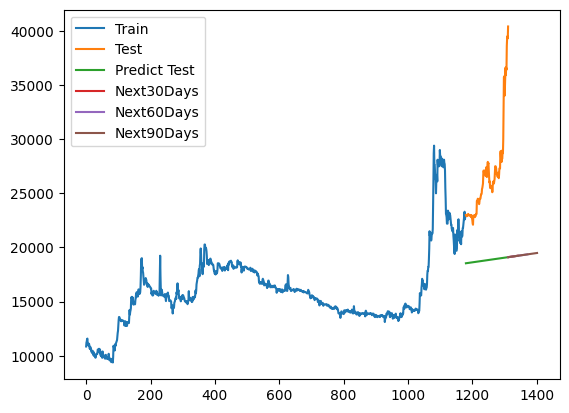
\includegraphics[width=\linewidth]{bibliography/Figure/LN_DHT(9_1).png}
    \caption{Linear model's result with 9:1 splitting proportion}
    \label{fig8}
  \end{minipage}
\end{figure}

\begin{figure}[H]
  \centering
  \begin{minipage}{0.8\linewidth}
    \centering
    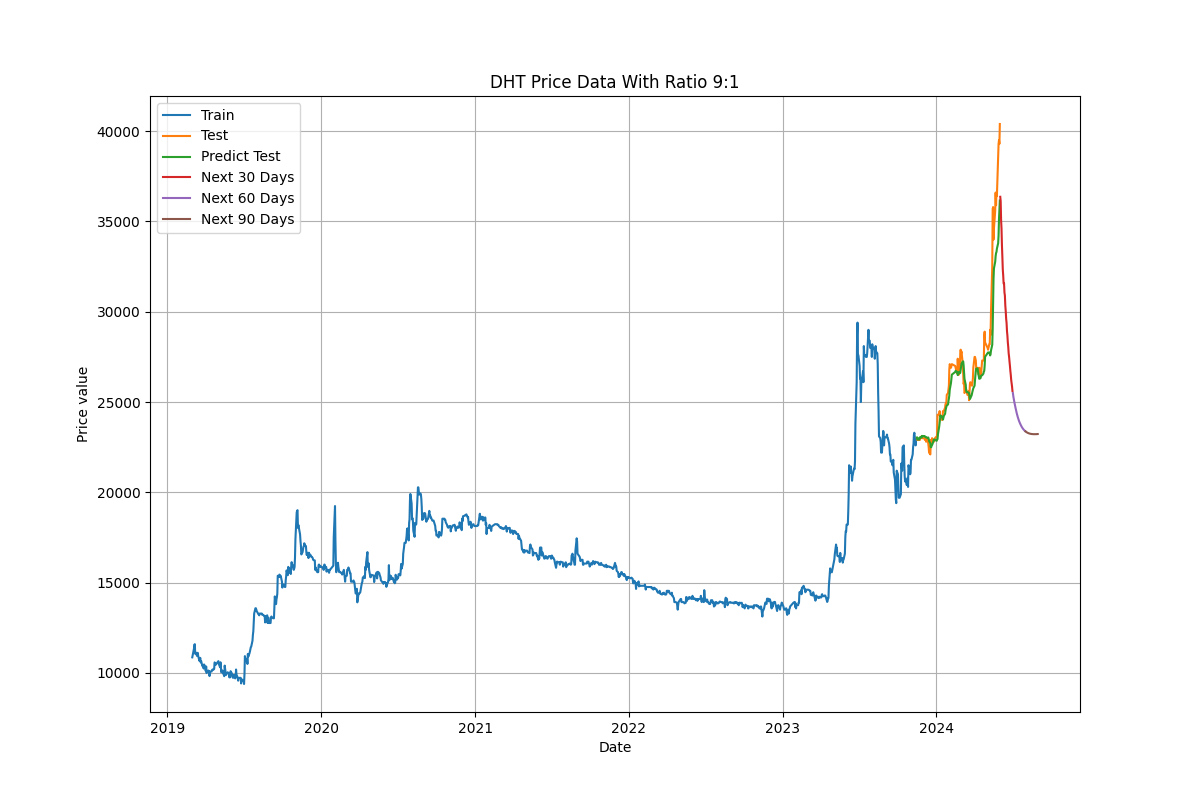
\includegraphics[width=\linewidth]{bibliography/Figure/RNN_91_DHT.png}
    \caption{RNN model's result with 9:1 splitting proportion}
    \label{fig8}
  \end{minipage}
\end{figure}

\begin{figure}[H]
  \centering
  \begin{minipage}{0.8\linewidth}
    \centering
    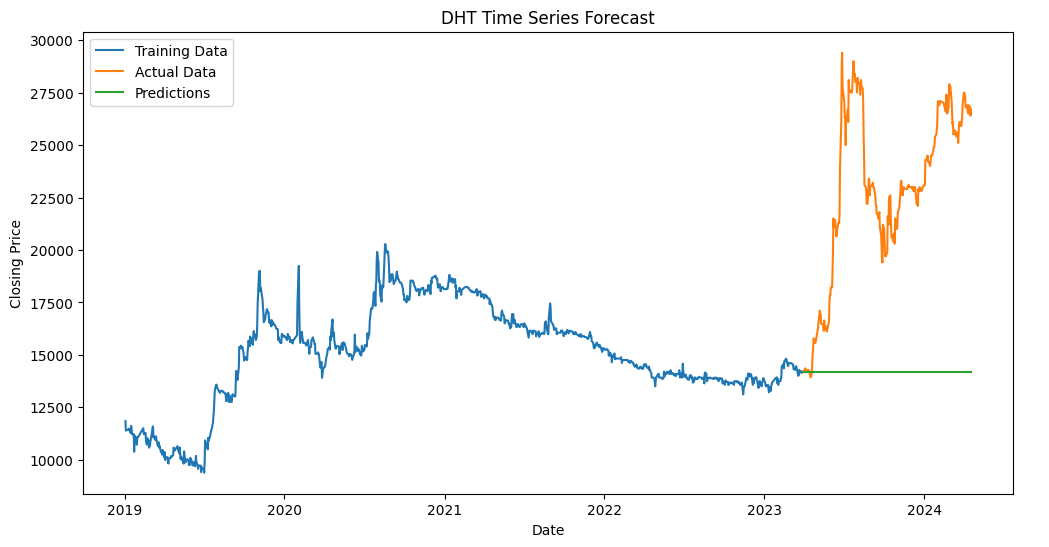
\includegraphics[width=\linewidth]{bibliography/Figure/DHT_ARIMA.png}
    \caption{Arima model's result with 8:2 splitting proportion}
    \label{fig8}
  \end{minipage}
\end{figure}

\begin{figure}[H]
  \centering
  \begin{minipage}{0.8\linewidth}
    \centering
    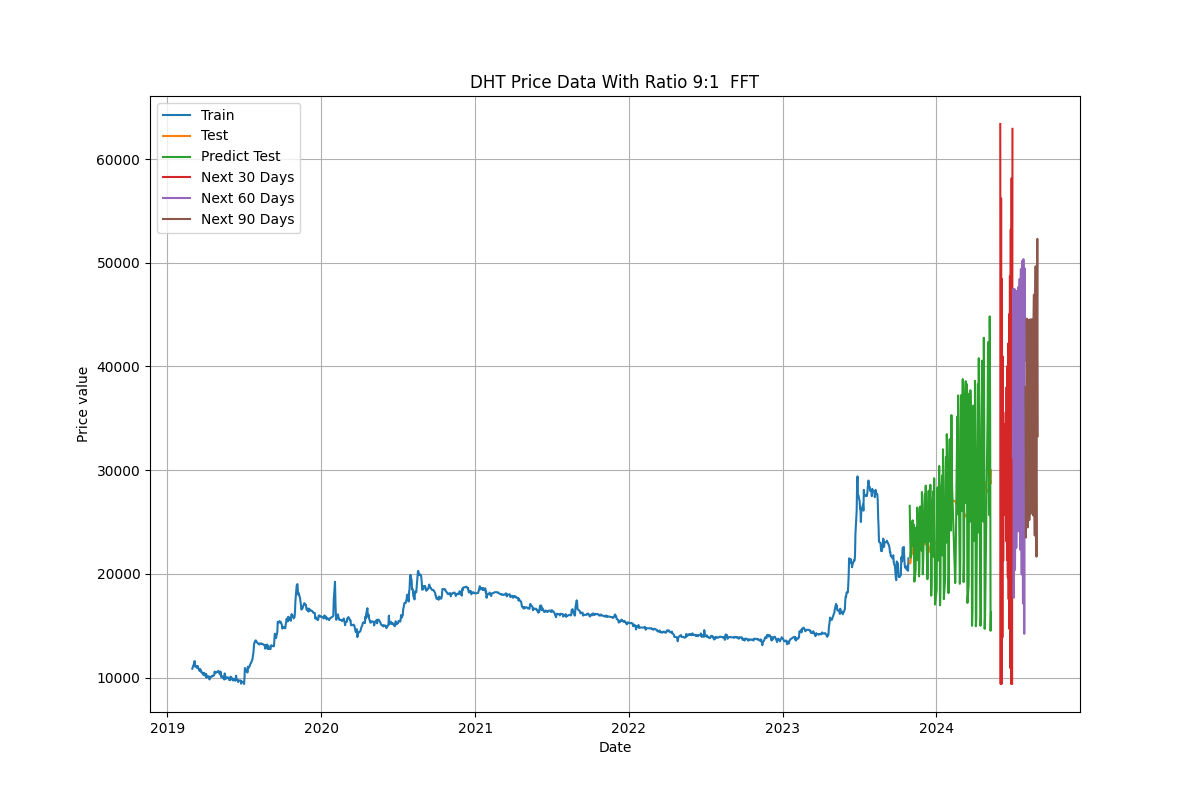
\includegraphics[width=\linewidth]{bibliography/Figure/FFT_91_DHT.png}
    \caption{FFT model's result with 9:1 splitting proportion}
    \label{fig8}
  \end{minipage}
\end{figure}

\begin{figure}[H]
  \centering
  \begin{minipage}{0.8\linewidth}
    \centering
    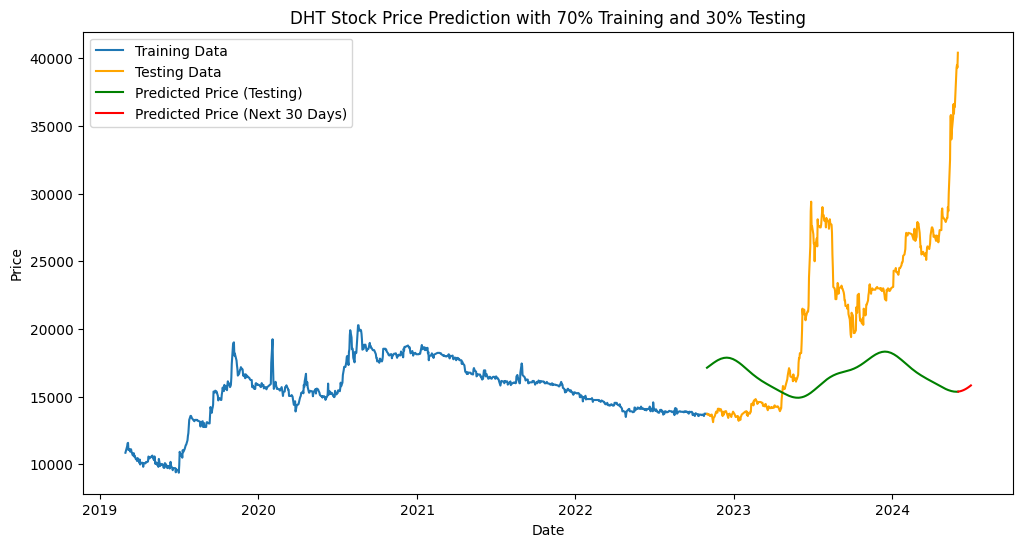
\includegraphics[width=\linewidth]{bibliography/Figure/DHT_LN_CF&DP.png}
    \caption{LN-CF-DP model's result with 7:3 splitting proportion}
    \label{fig8}
  \end{minipage}
\end{figure}

\begin{figure}[H]
  \centering
  \begin{minipage}{0.8\linewidth}
    \centering
    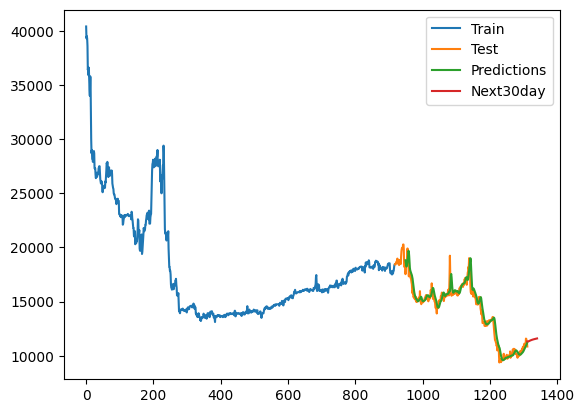
\includegraphics[width=\linewidth]{bibliography/Figure/LSTM_DHT(7_3).png}
    \caption{LSTM model's result with 7:3 splitting proportion}
    \label{fig8}
  \end{minipage}
\end{figure}

\begin{figure}[H]
  \centering
  \begin{minipage}{0.8\linewidth}
    \centering
    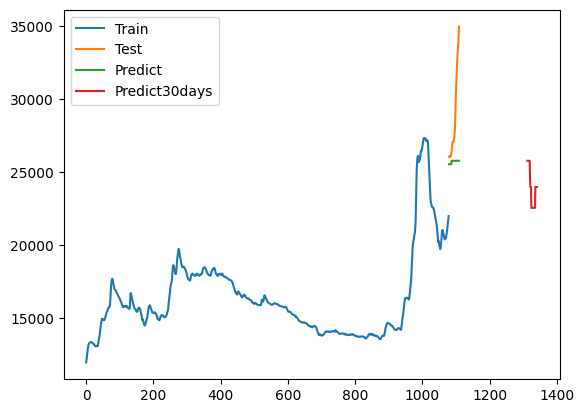
\includegraphics[width=\linewidth]{bibliography/Figure/LightGBM_DHT(8_2).png}
    \caption{LightGBM model's result with 8:2 splitting proportion}
    \label{fig8}
  \end{minipage}
\end{figure}

\begin{figure}[H]
  \centering
  \begin{minipage}{0.8\linewidth}
    \centering
    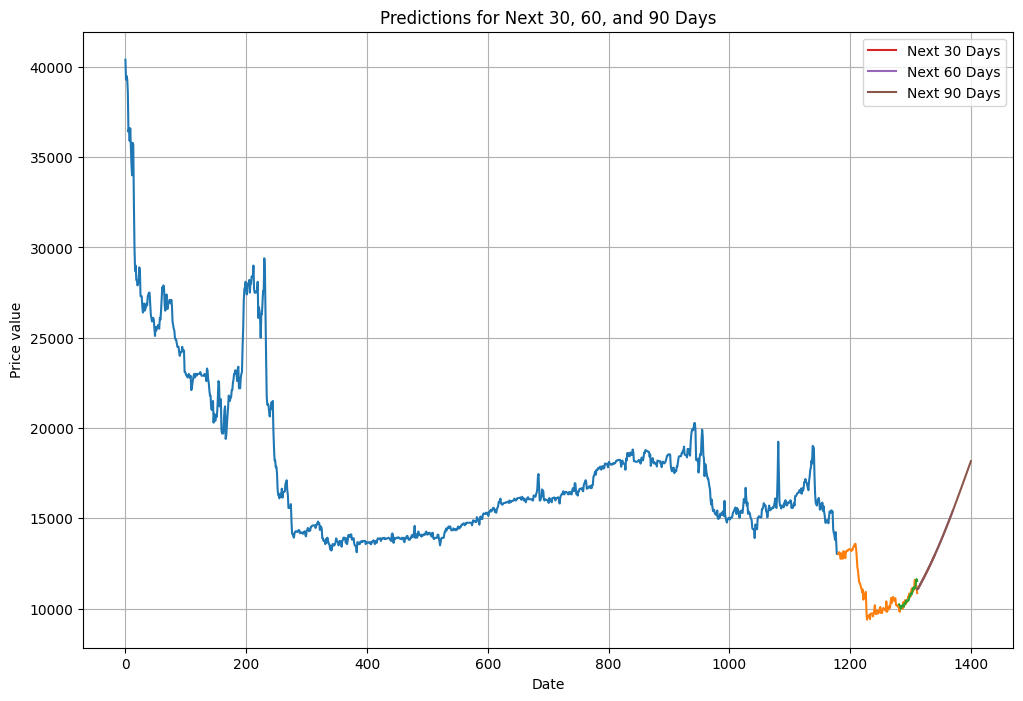
\includegraphics[width=\linewidth]{bibliography/Figure/DHT_GRU.png}
    \caption{GRU model's result with 8:2 splitting proportion}
    \label{fig8}
  \end{minipage}
\end{figure}

\section*{Acknowledgment}
\addcontentsline{toc}{section}{Acknowledgment}
We would like to express our sincere gratitude to \textbf{Assoc. Prof. Dr. Nguyen Dinh Thuan} and \textbf{Mr. Nguyen Minh Nhut} for their exceptional guidance, expertise, and invaluable feedback throughout the research process. Their meticulous mentoring and corrections, especially from Dr. Thuan, significantly shaped the direction and quality of this study. Mr. Nhut's dedicated guidance has been instrumental in our research journey.
\\This research would not have been possible without their support and contributions. We extend our heartfelt thanks to everyone involved for their invaluable assistance, encouragement, and belief in our research. We deeply appreciate their continuous support and guidance.

\section{CONCLUSION}

\subsection{SUMMARY}

This research explored various methods for predicting stock prices, ranging from traditional statistical models to advanced machine learning algorithms. The models tested include Linear Regression (LR), ARIMA, GRU, RNN, LSTM, FFT, LightGBM, and LN-CF-DP. Among these, LSTM and GRU stand out as the most effective models for stock price prediction.

Each model provides unique insights: deep learning models effectively capture non-linear patterns, traditional methods offer interpretable results, while LightGBM efficiently handles multiple data features.

Although no method can perfectly predict stock prices due to market complexities, this study provides a comprehensive toolkit for investors in the pharmaceutical sector.

\subsection{FUTURE CONSIDERATIONS}

To advance this research in the future, focus should be placed on:

\begin{enumerate}
    \item Optimizing existing models: Improve the accuracy of LightGBM, LSTM, and GRU through hyperparameter tuning and advanced data processing techniques.
    \item Incorporating sentiment analysis: Integrate data from pharmaceutical industry news and social media to capture the impact of market sentiment.
    \item Expanding data scope: Add macroeconomic indicators and pharmaceutical industry-specific data to enhance predictive capabilities.
    \item Applying ensemble learning techniques: Explore methods such as Bagging or Boosting to combine the strengths of multiple models.
    \item Researching new models: Monitor and experiment with the latest forecasting algorithms in machine learning and quantitative finance.
\end{enumerate}

By continuously exploring and incorporating new features, data sources, and modeling techniques, we can strive to continuously optimize forecasting models and enhance the ability to predict stock prices with greater accuracy and reliability.
%% UNCOMMENT these lines below (and remove the 2 commands above) if you want to embed the bibliografy.
\begin{thebibliography}{00}
\bibitem{1} Xiao, Y., \& Wang, J. (2017). A hybrid machine learning approach to stock price prediction. arXiv preprint arXiv:1708.05419.

\bibitem{2} Nelson, D. M., Pereira, A. C., \& de Oliveira, R. A. (2017). Stock market's price movement prediction with LSTM neural networks. In International joint conference on neural networks (pp. 1419-1426).

\bibitem{3} Bao, W., Yue, J., \& Rao, Y. (2017). A deep learning framework for financial time series using stacked autoencoders and long-short term memory. PloS one, 12(7), e0180944.

\bibitem{4} Minh, D. L., Sadeghi-Niaraki, A., Huy, H. D., Min, K., \& Moon, H. (2018). Deep learning approach for short-term stock trends prediction based on two-stream gated recurrent unit network. IEEE Access, 6, 55392-55404.

\bibitem{5} Chen, J., Li, K., Tang, Z., Bilal, K., Yu, S., Weng, C., \& Li, K. (2020). A parallel random forest algorithm for big data in a spark cloud computing environment. IEEE Transactions on Parallel and Distributed Systems, 32(1), 1-17.

\bibitem{6} Mamon, R. S., Arya, V., Kamalakannan, R., \& Gadde, S. (2021). Forecasting Stock Index Returns During COVID-19: Machine Learning Fusion Approach. Mathematics, 9(14), 1641.

\bibitem{7} Kostadinov, S. (2017, December 16). Understanding GRU networks. Towards Data Science. https://towardsdatascience.com/understanding-gru-networks-2ef37df6c9be.

\bibitem{8} Fuqua School of Business. (n.d.). Introduction to ARIMA models. Duke.edu. Retrieved June 20, 2024, from https://people.duke.edu/~rnau/411arim.htm

\bibitem{9} Nau, R. (2014). The mathematical structure of arima models. Duke University Online Article, 1(1), 1-8.



\end{thebibliography}
%%%%%%%%%%%%%%%


\EOD

\end{document}
